\subsection{Explicación formal del problema}
Sea $G=(V,E)$ un grafo simple conexo con $V=\{v_0, v_1, \dots, v_{n-1}\}$, $n\geq 2$, y $m$ aristas. Además sea $M\subseteq E$ tal que $M\neq \emptyset$. Se desea hallar un camino (no necesariamente simple) de $v_0$ a $v_{n-1}$ que pase al menos dos veces por un eje de $M$ (potencialmente el mismo) y que tenga longitud mínima.

En la figura (\ref{fig:ej-1.1}) pueden verse tres ejemplos. Los tres son muy parecidos pero permiten ilustrar distintas situaciones. En el primero (de izquierda a derecha y de arriba a abajo) encontramos el camino simple $P=(v_0,v_1,v_3,v_4,v_5)$ de longitud 4 que cumple con lo pedido pues tiene dos aristas especiales y es de longitud mínima. 

En el segundo se agregó una arista corriente entre los nodos $v_0$ y $v_5$. Puede notarse que en este caso el mejor camino es $P=(v_0,v_2,v_0,v_5)$ de longitud 3, el cual claramente no es simple pues pasa dos veces por el vértice $v_0$. 

En el último caso, la arista recientemente agregada pasa a ser especial. Al hacer esto tenemos dos caminos de longitud mínima entre los que pasan por dos aristas especiales: el $P$ que encontramos antes, y $P'=(v_0, v_5, v_0, v_5)$. Notar que $P'$ no solo no es simple, sino que también usa a $v_5$ como nodo intermedio. Cualquiera de los dos es igualmente aceptable.

\begin{figure}[H]
\begin{minipage}{0.5\textwidth}
\centering
\begin{tikzpicture}[shorten >=1pt,auto,node distance=1.9cm,
                    semithick]
  \tikzstyle{every state}=[fill=red,draw=none,text=white]

	\node[state, inner sep=3pt,minimum size=0pt, fill=blue]	(0)		 						  {$v_0$};
	\node[state, inner sep=3pt,minimum size=0pt]	(1) [right of=0, above of=0]  {$v_1$};
	\node[state, inner sep=3pt,minimum size=0pt]	(2) [right of=0, below of=0]  {$v_2$};
	\node[state, inner sep=3pt,minimum size=0pt]	(3) [right of=1] 						  {$v_3$};
	\node[state, inner sep=3pt,minimum size=0pt]	(4) [right of=3] 						  {$v_4$};
	\node[state, inner sep=3pt,minimum size=0pt, fill=blue]	(5) [below of=4, right of=4]  {$v_5$};
	\path	(0) edge 	[ultra thick]				node {} (1)
           	edge  [red]								node {} (2)
				(1) edge  [red, ultra thick]  node {} (3)
						edge	[ultra thick]				node {} (0)        
				(2) edge  [red]								node {} (0)
        (3)	edge  [red, ultra thick] 	node {} (4)
        		edge	[red, ultra thick]	node {} (1)
        (4) edge	[ultra thick]				node {} (5)
        		edge	[red, ultra thick]	node {} (3)
        (5) edge	[ultra thick]				node {} (4);

\end{tikzpicture}
\end{minipage}%
\begin{minipage}{0.5\textwidth}
\centering
\begin{tikzpicture}[shorten >=1pt,auto,node distance=1.9cm,
                    semithick]
  \tikzstyle{every state}=[fill=red,draw=none,text=white]

	\node[state, inner sep=3pt,minimum size=0pt, fill=blue]	(0)		 						  {$v_0$};
	\node[state, inner sep=3pt,minimum size=0pt]	(1) [right of=0, above of=0]  {$v_1$};
	\node[state, inner sep=3pt,minimum size=0pt]	(2) [right of=0, below of=0]  {$v_2$};
	\node[state, inner sep=3pt,minimum size=0pt]	(3) [right of=1] 						  {$v_3$};
	\node[state, inner sep=3pt,minimum size=0pt]	(4) [right of=3] 						  {$v_4$};
	\node[state, inner sep=3pt,minimum size=0pt, fill=blue]	(5) [below of=4, right of=4]  {$v_5$};
	\path	(0) edge 											node {} (1)
           	edge  [red, ultra thick]	node {} (2)
						edge 	[ultra thick]				node {} (5)
				(1) edge  [red]							  node {} (3)
						edge											node {} (0)        
				(2) edge  [red, ultra thick]	node {} (0)
        (3)	edge  [red]							 	node {} (4)
        		edge	[red]								node {} (1)
        (4) edge											node {} (5)
        		edge	[red]	node {} (3)
        (5) edge											node {} (4)
        		edge	[ultra thick]				node {} (0);

\end{tikzpicture}
\end{minipage}%

\vspace{15pt}
\centering
\begin{minipage}{0.5\textwidth}
\begin{tikzpicture}[shorten >=1pt,auto,node distance=2cm,
                    semithick]
  \tikzstyle{every state}=[fill=red,draw=none,text=white]

	\node[state, inner sep=3pt,minimum size=0pt, fill=blue]	(0)		 						  {$v_0$};
	\node[state, inner sep=3pt,minimum size=0pt]	(1) [right of=0, above of=0]  {$v_1$};
	\node[state, inner sep=3pt,minimum size=0pt]	(2) [right of=0, below of=0]  {$v_2$};
	\node[state, inner sep=3pt,minimum size=0pt]	(3) [right of=1] 						  {$v_3$};
	\node[state, inner sep=3pt,minimum size=0pt]	(4) [right of=3] 						  {$v_4$};
	\node[state, inner sep=3pt,minimum size=0pt, fill=blue]	(5) [below of=4, right of=4]  {$v_5$};
	\path	(0) edge 											node {} (1)
           	edge  [red]								node {} (2)
						edge 	[red, ultra thick]	node {} (5)
				(1) edge  [red]							  node {} (3)
						edge											node {} (0)        
				(2) edge  [red]								node {} (0)
        (3)	edge  [red]							 	node {} (4)
        		edge	[red]								node {} (1)
        (4) edge											node {} (5)
        		edge	[red]	node {} (3)
        (5) edge											node {} (4)
        		edge	[red, ultra thick]				node {} (0);

\end{tikzpicture}
\end{minipage}%
\caption{\footnotesize{Ejemplos del problema. Las aristas especiales están pintadas de rojo y las comunes de negro. Las aristas que pertenecen a la solución están engrosadas. En azul distinguimos a los nodos inicial y final.}}
  \label{fig:ej-1.1}
\end{figure}

\subsection{Explicación de la solución}
Si bien lo que se pide es, en definitiva, encontrar un camino mínimo en $G$, la dificultad adicional que implica hacer que el camino contenga al menos dos aristas de $M$ hace que no podamos aplicar de forma directa los algoritmos clásicos para este propósito. Para solventar esto consideraremos un grafo alternativo a $G$, $G'$, con el cual resolver el problema planteado originalmente será equivalente a encontrar un camino mínimo en $G'$ de forma tradicional (en este caso utilizando BFS).

\subsubsection{Construcción de $G'$}
Lo primero que haremos es armarnos un grafo nuevo $G'$ a partir de $G$. 

Consideramos tres grafos isomorfos a $G$: $G_0=(V_0,E_0)$, $G_1=(V_1,E_1)$ y $G_2=(V_2,E_2)$, tales que $f_k:V\rightarrow V_k/ f_k(v_i) = v_{k\times n + i}$ para $k\in \{0,1,2\}$ son las biyecciones correspondientes. En particular, $G_1 = G$. La figura (\ref{fig:ej-1.2}) ilustra la situación para un ejemplo puntual.

\begin{figure}[H]
\begin{minipage}{0.33\textwidth}
\centering
\begin{tikzpicture}[shorten >=1pt,auto,node distance=1.9cm,
                    semithick]
  \tikzstyle{every state}=[fill=red,draw=none,text=white]

	\node[state, inner sep=3pt,minimum size=0pt, fill=blue]	(0)		 						  {$v_0$};
	\node[state, inner sep=3pt,minimum size=0pt]	(1) [left of=0, below of=0]  {$v_1$};
	\node[state, inner sep=3pt,minimum size=0pt]	(2) [right of=0, below of=0]  {$v_2$};
	\node[state, inner sep=3pt,minimum size=0pt]	(3) [below of=1] 						  {$v_3$};
	\node[state, inner sep=3pt,minimum size=0pt]	(4) [below of=2] 						  {$v_4$};
	\node[state, inner sep=3pt,minimum size=0pt, fill=blue]	(5) [below of=4, left of=4]  {$v_5$};
	\path	(0) edge 											node {} (1)
           	edge  [red]								node {} (2)
				(1) edge  [red]							  node {} (3)
						edge											node {} (0)        
				(2) edge  [red]								node {} (0)
						edge											node {} (4)
        (3)	edge	[red]								node {} (1)
        		edge											node {} (5)
        (4) edge	[red]								node {} (5)
        		edge											node {} (2)
        (5) edge	[red]								node {} (4)
        		edge											node {} (3);

\end{tikzpicture}
\end{minipage}%
\begin{minipage}{0.33\textwidth}
\centering
\begin{tikzpicture}[shorten >=1pt,auto,node distance=1.9cm,
                    semithick]
  \tikzstyle{every state}=[fill=red,draw=none,text=white]

	\node[state, inner sep=3pt,minimum size=0pt, fill=blue]	(0)		 						  {$v_6$};
	\node[state, inner sep=3pt,minimum size=0pt]	(1) [left of=0, below of=0]  {$v_7$};
	\node[state, inner sep=3pt,minimum size=0pt]	(2) [right of=0, below of=0]  {$v_8$};
	\node[state, inner sep=3pt,minimum size=0pt]	(3) [below of=1] 						  {$v_9$};
	\node[state, inner sep=3pt,minimum size=0pt]	(4) [below of=2] 						  {$v_{10}$};
	\node[state, inner sep=3pt,minimum size=0pt, fill=blue]	(5) [below of=4, left of=4]  {$v_{11}$};
	\path	(0) edge 											node {} (1)
           	edge  [red]								node {} (2)
				(1) edge  [red]							  node {} (3)
						edge											node {} (0)        
				(2) edge  [red]								node {} (0)
						edge											node {} (4)
        (3)	edge	[red]								node {} (1)
        		edge											node {} (5)
        (4) edge	[red]								node {} (5)
        		edge											node {} (2)
        (5) edge	[red]								node {} (4)
        		edge											node {} (3);

\end{tikzpicture}
\end{minipage}%
\vspace{15pt}
\centering
\begin{minipage}{0.33\textwidth}
\begin{tikzpicture}[shorten >=1pt,auto,node distance=1.9cm,
                    semithick]
  \tikzstyle{every state}=[fill=red,draw=none,text=white]

	\node[state, inner sep=3pt,minimum size=0pt, fill=blue]	(0)		 						  {$v_{12}$};
	\node[state, inner sep=3pt,minimum size=0pt]	(1) [left of=0, below of=0]  {$v_{13}$};
	\node[state, inner sep=3pt,minimum size=0pt]	(2) [right of=0, below of=0]  {$v_{14}$};
	\node[state, inner sep=3pt,minimum size=0pt]	(3) [below of=1] 						  {$v_{15}$};
	\node[state, inner sep=3pt,minimum size=0pt]	(4) [below of=2] 						  {$v_{16}$};
	\node[state, inner sep=3pt,minimum size=0pt, fill=blue]	(5) [below of=4, left of=4]  {$v_{17}$};
	\path	(0) edge 											node {} (1)
           	edge  [red]								node {} (2)
				(1) edge  [red]							  node {} (3)
						edge											node {} (0)        
				(2) edge  [red]								node {} (0)
						edge											node {} (4)
        (3)	edge	[red]								node {} (1)
        		edge											node {} (5)
        (4) edge	[red]								node {} (5)
        		edge											node {} (2)
        (5) edge	[red]								node {} (4)
        		edge											node {} (3);

\end{tikzpicture}
\end{minipage}%
\caption{\footnotesize{Tres isomorfismos del grafo original, construidos de la forma indicada.}}
  \label{fig:ej-1.2}
\end{figure}


Además, definimos $M'$, un conjunto de arcos (aristas orientadas) de peso 1, como 

{\footnotesize$M'= \{(f_0(v), f_1(w))$ y $(f_0(w), f_1(v)) / (v,w)\in M\} \cup \{(f_1(v), f_2(w)) $ y $(f_1(w), f_2(v))/ (v,w)\in M\}$}

Por ejemplo, en la figura (\ref{fig:ej-1.2}) la arista $(v_0, v_2)\in M$. Entonces queremos que $M'$ tenga los arcos $(v_0, v_8)$, $(v_2, v_6)$, $(v_6, v_{14})$ y $(v_8, v_{12})$.
Observar que en $M'$ solo hay arcos que van de nodos de $G_0$ a nodos de $G_1$, y de $G_1$ a $G_2$. En ningún caso hay arcos de $G_t$ a $G_h$, con $h<t$; ni arcos que vayan directamente de $G_0$ a $G_2$.

Entonces hasta acá tenemos tres grafos conexos isomorfos. Podemos pensarlos como las tres componentes conexas de un grafo con $3n$ vértices y $3m$ aristas. A continuación uniremos estas tres componentes mediante los arcos de $M'$: sea $G^*=(V_1\cup V_2\cup V_3, E_1\cup E_2\cup E_3 \cup M')$. 

Podemos pensar a $G^*$ con la siguiente analogía: cada una de las tres componentes es un nivel, y los arcos ``escaleras mecánicas'' que permiten subir de un nivel al siguiente en forma unidireccional y que no se saltea niveles. En este contexto, $G_k$ será el nivel $k$. Notar que entonces $G^*$ no es fuertemente conexo pues desde un nodo del nivel 2 o 3 no puedo alcanzar a un nodo en el nivel 1. Sin embargo, para cualquier vértice en el nivel 1 todos los vértices del grafo son alcanzables. En particular esto vale para $v_0$.  

\pgfmathsetmacro\angFuite{170}
\pgfmathsetmacro\coeffReduc{1.2}
\pgfmathsinandcos\sint\cost{\angFuite}

\begin{figure}
\centering
\begin{tikzpicture}[current plane/.estyle=%
        {cm={1,0,\coeffReduc*\cost,-\coeffReduc*\sint,(0,#1)}}, rotate=-5]

	\GraphInit[vstyle=Shade]

		\begin{scope}[current plane=0 cm, rotate=10]
			\SetVertexNoLabel
		  \SetGraphShadeColor{white}{teal}{gray}
		  \grEmptyCycle[Math,prefix=a]{6}
		\end{scope}

		\begin{scope}[current plane=4 cm, rotate=10]
			\SetVertexNoLabel
		  \SetGraphShadeColor{white}{teal}{gray}
		  \grEmptyCycle[Math,prefix=b]{6}
		\end{scope}

		\begin{scope}[current plane=8 cm, rotate=10]
			\SetVertexNoLabel
		  \SetGraphShadeColor{white}{teal}{gray}
		  \grEmptyCycle[Math,prefix=c]{6}
		\end{scope}

	\AssignVertexLabel[Math]{a}{v_3,v_1,v_0,v_2,v_4,v_5}
	\AssignVertexLabel[Math]{b}{v_9,v_7,v_6,v_8,v_{10},v_{11}}
	\AssignVertexLabel[Math]{c}{v_{15},v_{13},v_{12},v_{14},v_{16},v_{17}}

	\SetGraphShadeColor{white}{teal}{gray}
	\Edge(a0)(a5)
	\Edge(b0)(b5)
	\Edge(a2)(a1)
	\Edge(b2)(b1)
	\Edge(a3)(a4)
	\Edge(b3)(b4)
	\EdgeInGraphLoop{c}{6}

	\tikzset{EdgeStyle/.append style={dotted}}
	\Edge(a2)(a3)
	\Edge(b2)(b3)
	\Edge(a1)(a0)
	\Edge(b1)(b0)
	\Edge(a4)(a5)
	\Edge(b4)(b5)

	\SetGraphShadeColor{white}{red}{red}
	\tikzset{EdgeStyle/.append style={->, solid}}
	\Edge(a1)(b0)
	\Edge(b1)(c0)
	\tikzset{EdgeStyle/.append style={bend left=10}}
	\Edge(a2)(b3)
	\Edge(b2)(c3)
	\Edge(a4)(b5)
	\Edge(b4)(c5)
	\tikzset{EdgeStyle/.append style={<-, opacity=.3, bend left=0}}
	\Edge(b1)(a0)
	\Edge(c1)(b0)
	\tikzset{EdgeStyle/.append style={bend left=10}}
	\Edge(b2)(a3)
	\Edge(c2)(b3)
	\Edge(b4)(a5)
	\Edge(c4)(b5)
	
\end{tikzpicture}
\caption{$G'$ para el ejemplo dado en la figura (\ref{fig:ej-1.2}). Las líneas punteadas señalan las aristas que estaban en $G^*$ pero que quitamos.}
\label{fig:ej-1.3}
\end{figure}

Finalmente, definimos a $G'$ como el resultado de quitarle a los niveles 0 y 1 de $G^*$ todas las ``aristas isomorfas'' a las aristas de $M$.\footnote{En rigor, tanto $G'$ como $G^*$ sirven a nuestro propósito, pero $G'$ tiene la ventaja de que permitirá reducir el uso de memoria (potencialmente mucho si hay muchas aristas especiales) y constantes en la complejidad de la implementación.}

En este caso ya no es cierto que cualquier vértice de $G'$ sea alcanzable desde cualquier vértice del primer nivel: en efecto, si vemos la figura (\ref{fig:ej-1.3}), el nodo $v_2$ no es alcanzable desde el $v_0$. No obstante, sigue valiendo el siguiente lema:

\paragraph*{Lema 1.1: }Todo vértice del tercer nivel (nivel 2) de $G'$ es alcanzable desde todo vértice del primer nivel (nivel 0). 

\paragraph*{Demostración: }Sean $u,w\in V_1$ (es decir, ambos del nivel 0). Supongamos que $w$ no es alcanzable desde $u$ en $G'$. Como $G_1$ inicialmente era conexo, esto significa que existía camino de $u$ a $w$, $Q$, y seguro incluía alguna arista especial (sino seguiría existiendo en $G'$ y $w$ sería alcanzable desde $u$). Como todos los nodos que eran incidentes a una arista especial en $G_1$ son incidentes a un arco en $G'$, seguro existe $z\in Q$, tal que $z$ es incidente a un arco que permite pasar al segundo nivel. Luego, es posible llegar desde $u$ a algún vértice del segundo nivel. Si no existe tal nodo $w$, entonces cualquier nodo del primer nivel es alcanzable desde $u$, y como $M$ no era vacío, entonces seguro hay un camino desde $u$ hasta el segundo nivel.

Es fácil ver que exactamente el mismo razonamiento se puede realizar para probar que es posible llegar desde cualquier nodo del segundo nivel a algún nodo del tercer nivel. Luego, por concatenación de ambas cosas, es posible llegar desde cualquier nodo del primer nivel a algún nodo del tercero. Pero como el tercer nivel sigue siendo conexo (pues nunca quitamos las aristas especiales) entonces es claro que esto es equivalente a poder llegar a cualquier nodo del tercer nivel. $\qed$

Debido a este lema, y como todas las aristas de $G'$ tienen peso 1, es posible aplicar el algoritmo BFS para hallar el camino mínimo entre un nodo del nivel 0 y otro del 2. Particularmente, entre los nodos 0 y $3n-1$. 

En la sección siguiente probaremos que esto es equivalente a resolver el problema planteado originalmente.

\subsubsection{Correctitud y optimalidad}
La siguiente proposición garantiza la correctitud y optimalidad de nuestra solución.

\paragraph*{Proposición 1.1: } 
Sea $P'=(v_0, v_{i_1},\dots, v_{i_p}, v_{3n-1})$ un camino mínimo de $v_0$ a $v_{3n-1}$ en $G'$, entonces $P = P'$ mod $n$ \footnote{$P = P'$ mod $n \Leftrightarrow P_i = v_{j\text{ mod }n}\text{ donde $P'_i=v_j$ }, i = 0,\dots, k-1$} es camino de $v_0$ a $v_{n-1}$ en G, mínimo entre los que pasan por al menos dos aristas especiales.

\paragraph*{Demostración: }

Hay que ver tres cosas respecto de $P$: que es camino de $v_0$ a $v_{n-1}$, que pasa por al menos dos aristas especiales, y que es mínimo respecto a los caminos que cumplen ambas cosas.

Va a ser útil recordar que $f_k:V\rightarrow V_k/ f_k(v_i) = v_{k\times n + i}$ para $k\in \{0,1,2\}$ son las biyecciones de los isomorfismos planteados en la sección anterior. Además una pequeña observación que usaremos fuertemente: 

\paragraph*{Observación 1.1: }$G=(V,E)$. $(u,w)\in E$ pero $(u,w)\notin M$ si y solo si $(f_0(u), f_0(w)), (f_1(u), f_1(w))$ y $(f_2(u), f_2(w))$ son aristas de $G'$. \\
En cambio, $(u,w)\in M$ si y solo si los arcos $(f_0(u), f_1(w)),$ $(f_0(w), f_1(u)), (f_1(u), f_2(w))$ y $(f_1(w), f_2(u))$ están en $G'$. \\
Ambas cosas valen por como construimos $G'$.

\begin{itemize}
	\item Es camino: Ante todo, por definición del operador módulo vale que
	\begin{center}
		$(\forall v_i\in P)$ $0\leq i$ mod $n\leq n-1$
	\end{center}

	 Es decir que todos los vértices de $P$ pertenecen a $G$, y además empieza en $v_0$ y termina en $v_{n-1} = v_{(3n-1)\text{ mod } n}=v_{(2n+n-1)\text{ mod } n} $. Queda ver que efectivamente nodos consecutivos en $P$ son adyacentes en $G$. \\Si $v_i, v_j\in P$ son consecutivos entonces $v_{h+i}\in P'$ tiene que ser adyacente con $v_{h'+j}\in P'$ (pues son nodos consecutivos en un camino), donde $h$ y $h'$ son un par de constantes múltiplos de $n$. Por el contexto del problema $h$ y $h'$ solo pueden ser $0, n$ o $2n$. Luego, si $h=h'=k\times n$, por la observación 1.1, si $v_{h+i}$ es adyacente a $v_{h+j}$ en $G_k$ (cosa que pasa, sino no podría pasar en $G'$) entonces $v_i$ es adyacente a $v_j$ en $G$. Si $h\neq h'$, seguro que cada nodo es el extremo de un arco (pues están en diferentes niveles). Pero por construcción de $G'$, solo puede haber un arco entre $v_{h+i}$ y $v_{h'+j}$ si había una arista especial entre $v_i$ y $v_j$ en $G$, lo que significa que eran adyacentes. Luego, queda probado que $P$ es un camino válido de $v_0$ a $v_{n-1}$.
	\item Pasa por al menos dos aristas especiales: el nodo $v_{3n-1}$ pertenece al nivel 2 de $G'$. Esto significa que paso por dos arcos. Un arco entre $v_{k\times n + i}$ y $v_{(k+1)\times n + j}$ en $G'$ solo existe si $(v_i, v_j)\in M$. Por definición de $P$, si tal arco pertenece a $P'$ entonces tal arista especial pertenece a $P$. Luego, $P$ tiene al menos dos aristas de $M$ (podría tener más, pues en el tercer nivel las aristas especiales siguen existiendo y no son arcos).
	\item Es mínimo: Supongamos que $P$ no es óptimo para el problema. Entonces existe $Q$ tal que $|Q| < |P|$ y cumple con pasar por dos aristas de $M$. Construyamos $Q'$, un camino de $v_0$ a $v_{3n-1}$ en $G'$, basado en $Q$.\\
	El método propuesto a continuación para armar $Q'$ hace uso fuertemente de la observación 1.1, pues esta nos garantiza que las aristas y arcos mencionados efectivamente existen en $G'$.\\
	 La idea es la siguiente: recorremos las aristas de $Q$ en orden y las vamos poniendo en $Q'$ hasta encontrar la primer arista especial, $(v_i, v_j)$. En su lugar agregamos el arco $(v_i, v_{n+j})$ $=(f_0(v_i), f_1(v_j))$ a $Q'$. Seguimos completando $Q'$ con aristas $(f_1(u), f_1(w))$ por cada arista común $(u,w)$ que encontramos en $Q$. Eventualmente llegamos a una segunda arista especial (por hipótesis existe), $(v_s, v_t)$, y en su lugar agregamos el arco $(v_{n+s}, v_{2n+t}) = (f_1(v_s), f_2(v_t))$ a $Q'$. Ahora bien, en este punto si $Q$ es mínimo lo mejor que puede hacer es tomar el camino de distancia mínima desde $v_t$ hasta $v_{n-1}$. Pero tal camino es isomorfo a un camino desde $v_{2n+t}=f_2(v_t)$ hasta $v_{3n-1}=f_2(v_{n-1})$, pues el tercer nivel es isomorfo a $G$. Por lo tanto agregando este camino a $Q'$, llegamos a que $Q'$ es un camino de $v_0$ a $v_{3n-1}$ en $G'$. \\
	 Pero como $|Q'|=|Q|<|P|=|P'|$, encontramos un camino más corto que $P'$ en $G'$ tal que conecta los mismos vértices. Esto es absurdo, pues por hipótesis $P'$ era camino mínimo. Luego, el absurdo provino de suponer que $P$ no era óptimo para el problema.
\end{itemize}

Finalmente, queda demostrada la proposición. $\qed$

De hecho, la recíproca de esta proposición también vale. No lo probamos sin embargo porque no es necesario para la correctitud de la solución. La forma de probarlo sería similar igualmente.

\subsubsection{Explicación del código}

Notar que para las dimensiones del grafo que toma BFS no usamos $n$ y $m$ sino $n'$ y $m'$, para no confundir con las dimensiones del problema original puesto que pueden ser diferentes, y de hecho por cómo lo vamos a usar, así va a ser.

\begin{algorithm}[H]
  \begin{algorithmic}[1]
  \caption{Pseudocódigo del procedimiento BFS}
  \label{algo:1-1}
    \Procedure{bfs}{\texttt{ListaAdyacencia} $vs$, \texttt{vertice} $root$, \texttt{vertice} $target$, \texttt{int} $n'$}$\rightarrow$ \texttt{Vector<vertice>}
    	\State \texttt{cola<vertice>} $c \gets Vacia()$
    	\Comment $O(1)$
    	\State \texttt{vector<int>} $distancia(n', \infty)$
    	\Comment $O(n')$
    	\State \texttt{vector<vertice>} $acm(n', -1)$
    	\Comment $O(n')$
    	\State $distancia[root]\gets 0$
    	\Comment $O(1)$
    	\State $acm[root]\gets root$
    	\Comment $O(1)$
    	\State $c.push(root)$
    	\Comment $O(1)$
    	\While{$\neg c.vacia?()$}
    		\Comment $O(n)$ veces
    		\State $actual\gets c.pop()$
    		\Comment $O(1)$
    		\State \texttt{VerticesAdyacentes} $vecinos\gets vs[actual]$
    		\Comment $O(1)$
    		\For{$v \in vecinos$}
    		\Comment $O(d(v))$ veces
    			\If{$distancia[v] = \infty$}
    			\Comment $O(1)$
    				\State $distancia[v]\gets distancia[actual] + 1$
    				\Comment $O(1)$
    				\State $acm[v] = actual$
    				\Comment $O(1)$
    				\If{$v=target$}
    				\Comment $O(1)$
    					\State $break$
    					\Comment $O(1)$
    				\EndIf
    				\State $c.push(v)$
    				\Comment $O(1)$
    			\EndIf
    		\EndFor
    	\EndWhile
    	\State \texttt{int} $long\_sol\gets distancia[target]-1$
    	\Comment $O(1)$
    	\State \texttt{vector<vertice>} $solucion(long\_sol, 0)$
    	\Comment $O(long\_sol)\subseteq O(m')$
    	\State \texttt{vertice} $v\gets acm[target]$
    	\Comment $O(1)$
    	\For{\texttt{int} $i$ desde $long\_sol - 1$ hasta $0$}
    	\Comment $O(m')$ veces
    		\State $solucion[i]\gets v$
    		\Comment $O(1)$
    		\State $v\gets acm[v]$
    		\Comment $O(1)$
    	\EndFor
    	\State \texttt{return} $solucion$
		\EndProcedure
	\end{algorithmic}
\end{algorithm}

La implementación de BFS que realizamos está compuesta por dos partes: la primera hasta la línea 17 inclusive, es la implementación clásica del algoritmo de búsqueda en anchura para determinar caminos mínimos, en particular modificada un poco para que termine a penas compute un camino hasta el nodo objetivo pues es el único que nos importa realmente; la segunda consiste en reconstruir el camino mínimo entre $root$ y $target$ a partir del árbol de caminos mínimos. Notar que la función tiene como precondición que efectivamente exista algún camino desde $root$ hasta $target$.

Para la primer parte tenemos esencialmente tres estructuras importantes: 
\begin{itemize}
\item una cola FIFO de vértices donde iremos encolando los vecinos del nodo en el que estamos actualmente y que todavía no hayamos visitado; la misma está implementada sobre una lista doblemente enlazada, lo que permite que las operaciones de encolar, desencolar y ver el siguiente elemento sean todas $O(1)$.
\item un vector de distancias tal que la posición i-ésima del mismo guarda la distancia desde el $root$ hasta el nodo $i$ (o bien $\infty$ si todavía no pasamos por $i$, o simplemente $i$ no es alcanzable desde $root$).
\item un vector de vértices que representará nuestro árbol de caminos mínimos desde el $root$ hasta cualquier nodo, de forma que en la posición i-ésima del vector tendremos al padre del nodo $i$ en el árbol (o bien -1, si todavía no pasamos por $i$, o simplemente no es alcanzable desde $root$).
\end{itemize}

Que la búsqueda es correcta es resultado inmediato de que el algoritmo es el BFS tradicional cuya correctitud es conocida. Una discusión más detallada de este algoritmo junto con una demostración de su correctitud puede encontrarse en \cite[Ch. 22.2]{cormen}.

Una vez hallado un camino mínimo hasta el nodo $target$, queremos ahora armar un vector de vértices que contenga a todos los vértices de dicho camino. Como la distancia es la cantidad de vértices en el camino menos uno, entonces el vector tendrá que tener tamaño igual a la distancia más uno. Pero como no nos interesa que el primer y último nodos estén en el vector entonces nos queda que el largo del mismo será $l=d(root, target) - 1$. Luego, es cuestión de llenar las posiciones de este vector de atrás para adelante, pues \emph{a priori} para cada nodo solo sabemos cual es su padre en el árbol de caminos mínimos. La última posición tendrá al padre del nodo $target$, la anteúltima al padre del padre y así. Iterando $l$ veces llegamos a que en la posición inicial del vector hay un nodo que es hijo de $root$ y ancestro de $target$.

Finalmente devolvemos este vector.

\begin{algorithm}[H]
  \begin{algorithmic}[1]
  \caption{Pseudocódigo del main}
  \label{algo:1-2}
    \Procedure{main}{}
    	\State \texttt{int} $n$
    	\Comment {Cantidad de nodos}
    	\State \texttt{vector(vector(int))} $input$
    	\Comment {\small $input[i]$ almacena los datos de la i-ésima arista pasada}\normalsize
    	\State $inicializar(input, n)$
    	\Comment \small Leemos los datos pasados como parámetros e inicializamos \normalsize
    	\State \texttt{ListaAdyacencia} $adj\_list(3*n, VerticesAdyacentes()$)
    	\Comment $O(3\times n) = O(n)$
    	\For{$(v_1, v_2, e) \in input$}
    	\Comment $m$ veces
    		\If{$e = True$}
    		\Comment $O(1)$
    			\State $adj\_list[v_1].push\_back(v_2 + n)$
    			\Comment $O(1)$
    			\State $adj\_list[v_1 + n].push\_back(b + 2\times n)$
    			\Comment $O(1)$
    			\State $adj\_list[v_2].push\_back(v_1 + n)$
    			\Comment $O(1)$
    			\State $adj\_list[v_2 + n].push\_back(v_1 + 2\times n)$
    			\Comment $O(1)$
    		\Else
     			\State $adj\_list[v_1].push\_back(v_2)$
     			\Comment $O(1)$
     			\State $adj\_list[v_2].push\_back(v_1)$
     			\Comment $O(1)$
     			\State $adj\_list[v_1 + n].push\_back(v_2 + n)$
     			\Comment $O(1)$
     			\State $adj\_list[v_2 + n].push\_back(v_1 + n)$
     			\Comment $O(1)$
    		\EndIf
    		\State $adj\_list[v_1 + 2\times n].push\_back(v_2 + 2\times n)$
    		\Comment $O(1)$
    		\State $adj\_list[v_2 + 2\times n].push\_back(v_1 + 2\times n)$
    		\Comment $O(1)$
    	\EndFor
    	\State \texttt{vector<vertice>} $solucion\gets bfs(adj\_list, 0, 3\times n)$
    	\Comment $O(3n + 6m) = O(n + m)$
    	\State $print(solucion.size() + 1)$
    	\For{$v \in solucion$}
    		\State $print(v \% n)$
    	\EndFor
		\EndProcedure
  \end{algorithmic}
  \end{algorithm}

Nuestra función main tiene tres partes importantes:
\begin{itemize}
	\item El armado de la lista de adyacencias de $G'$. Si la arista que estamos agregando es especial, agregamos los arcos correspondientes del nivel 0 al 1, y del 1 al 2. Si no lo es, entonces agregamos la arista tanto en el nivel 0 como en el 1. En ambos casos, agregamos la arista normalmente en el nivel 2.
	\item El llamado a BFS pasando como parámetros la lista de adyacencias anterior, tomando como $root$ el nodo $0$ y como target el $3n-1$. Dichos parámetros cumplen las precondiciones de BFS por el Lema 1.1 y por ser todas aristas de peso 1.
	\item La impresión del resultado. Acá es importantísimo notar que imprimimos los vértices módulo $n$ pues lo que nos devuelve BFS son nodos del grafo $G'$ y no de $G$. Por la Proposición 1.1 esto efectivamente constituye una solución al problema original.
\end{itemize}

\subsection{Complejidad del algoritmo}
La complejidad en peor caso de la solución es la complejidad de la función $main$. Omitiendo las partes de lectura y escritura de datos, tenemos que el costo de dicha función es el costo de armar el nuevo grafo más el costo de realizar $BFS$ sobre él.

Viendo el algoritmo \ref{algo:1-2}, el costo de armar el grafo es $O(n+6m) = O(n+m)$. Vale destacar que esta complejidad es además claramente una cota inferior, pues el costo de armar el grafo nuevo depende únicamente de la cantidad de vértices y aristas, y no de características más particulares como la cantidad de aristas especiales, la longitud de los caminos simples, etc. Por lo tanto el algoritmo en general debe ser al menos $\Omega(n+m)$.

Por otra parte, observando el algoritmo \ref{algo:1-1}, $BFS$ tiene una complejidad en peor caso de 

\begin{equation}
\begin{aligned}
	O(1+2n'+3+2n'+(\sum_{i=0}^{n'-1}d(v_{i}))\times 5 + m' + 1 + 2m') & = O(5+4n'+2m'\times 5 + 3m') \\
	&= O(4n'+13m') \\
	&= O(n'+m')
\end{aligned}
\end{equation}

Notar que en el primer término podemos escribir la sumatoria de los grados de todos los nodos debido a que en peor caso hará falta pasar por todos ellos, y por otra parte sabemos que pasamos por cada uno exactamente una vez. El segundo término resulta de agrupar y reemplazar la sumatoria por $2m'$ (cosa que podemos hacer pues es una identidad válida para todos los grafos).

En nuestro problema concreto $n'=3\times n$ y $m' = 2\times 3\times m = 6\times m$ (por cada arista que sacamos estamos poniendo dos arcos).

Luego, la complejidad asintótica del algoritmo en peor caso es $O(n+m+3n+6m) = O(4n+7m) = O(n+m)$. Por otra parte como dijimos que también era $\Omega(n+m)$, tenemos que es $\Theta(n+m)$.

De hecho, asintóticamente también lo es en mejor caso (cuando existe un camino de longitud 3): si bien $BFS$ puede ser $\Theta(1)$ debido a que nuestra implementación termina de buscar una vez que encuentra al nodo deseado, armar el grafo sigue siendo $\Theta(n+m)$ en cualquier caso. En definitiva no tiene sentido hablar de mejor o peor caso pues ambos son iguales en términos asintóticos.

\subsection{Performance del algoritmo}


Como dijimos anteriormente, el algoritmo tiene una complejidad de $\Theta(n + m)$. El algoritmo no tiene peor o mejor caso propiamente dichos (dado que es $\Theta(n + m)$ para todos los casos), pero veremos que, tomando $n$ fijo y moviendo $m$, podemos hacer variar el tiempo que toma el algoritmo.



\begin{figure}[H]
 \centering
	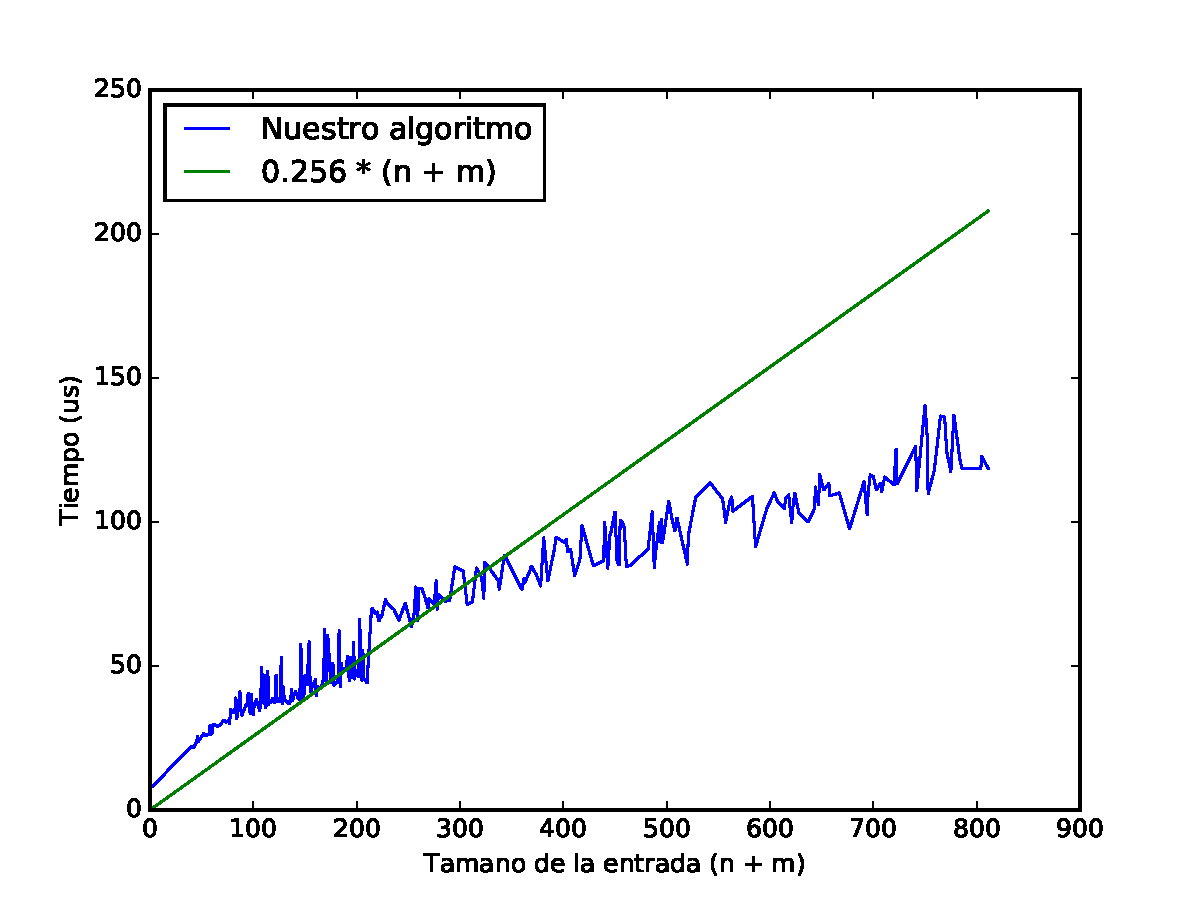
\includegraphics[width=0.9\textwidth]{img/exp/problema1-promedio.pdf}
	\caption{\footnotesize Tiempo que toma el algoritmo en $\mu$s para una entrada de tamaño $n + m$. $m$ al azar entre $n-1$ y $\frac{n(n-1)}{2}$.}
	\label{fig:problema1-promedio}
\end{figure}

Como se observa, la implementación tiene complejidad lineal sobre $n + m$, como era esperado.

Para confirmarlo, usamos el gráfico de la funcion $\frac{T(n + m)}{n + m}$, donde $T$ es el tiempo que tarda el algoritmo para la entrada de tamaño dado.
Si vemos que converge a una constante, estaremos en el caso exacto de la definción de $\Theta(f(n))$.

\begin{figure}[H]
 \centering
	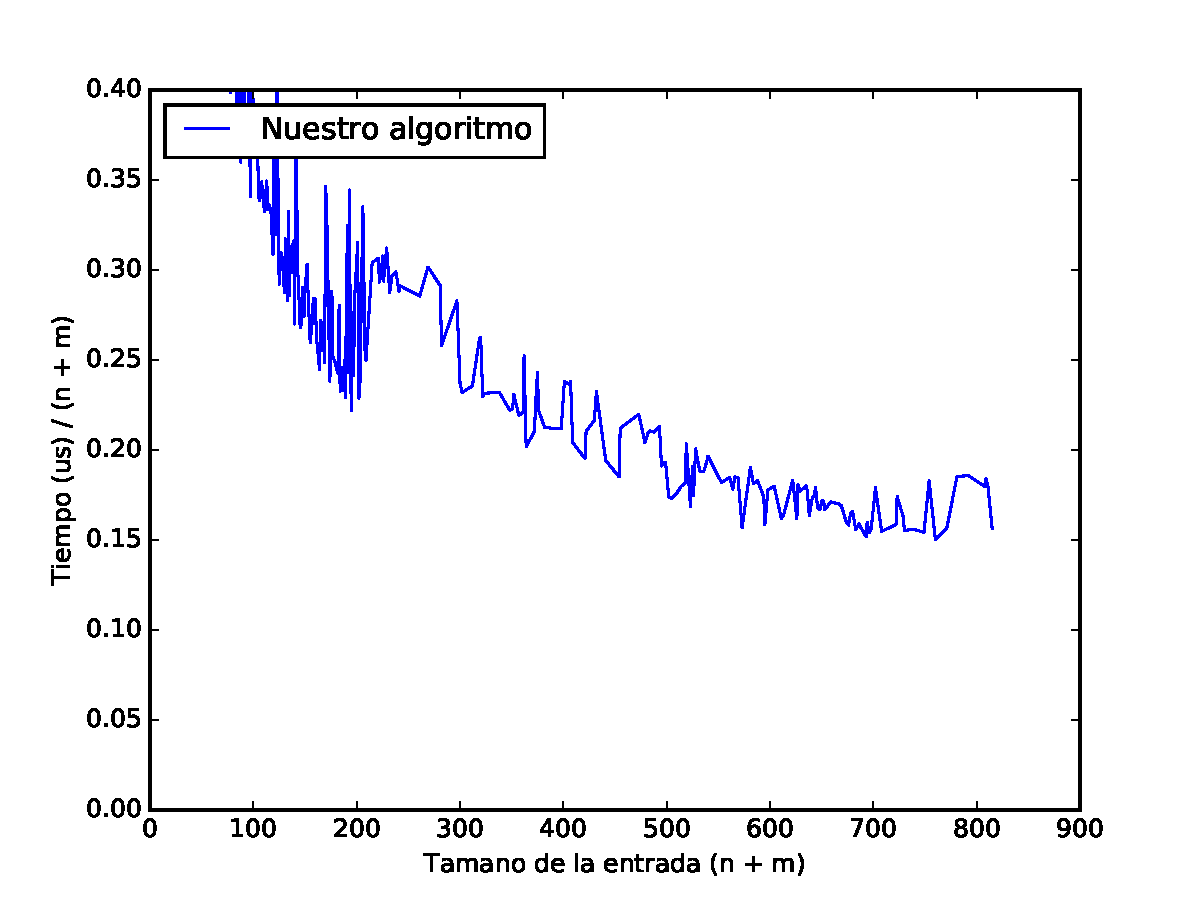
\includegraphics[width=0.9\textwidth]{img/exp/problema1-promedio2.pdf}
	\caption{\footnotesize Tiempo que toma el algoritmo en $\mu$s dividido $n + m$ para una entrada de tamaño $n + m$.  $m$ al azar entre $n-1$ y $\frac{n(n-1)}{2}$}
	\label{fig:problema1-promedio2}
\end{figure}

El ruido del gráfico se debe a que la escala es otra y distorciona las distancias entre los puntos. Sin embargo, se puede observar que converge a una constante, como era esperado.


Como habiamos dicho anteriormente, aunque el algoritmo es $\Theta(n + m)$, podemos ver casos particulares del algoritmo, en el que $n$ está fijo y movemos $m$ y ver como se comporta el algoritmo.

Primero veamos el caso en el que $m \in O(n)$. Esperaríamos que el algoritmo aquí tenga una complejidad de $O(n + m) = O(n + n) = O(n)$. Esto fue confirmado experimentalmente, como se muestra a continuación.

\begin{figure}[H]
 \centering
	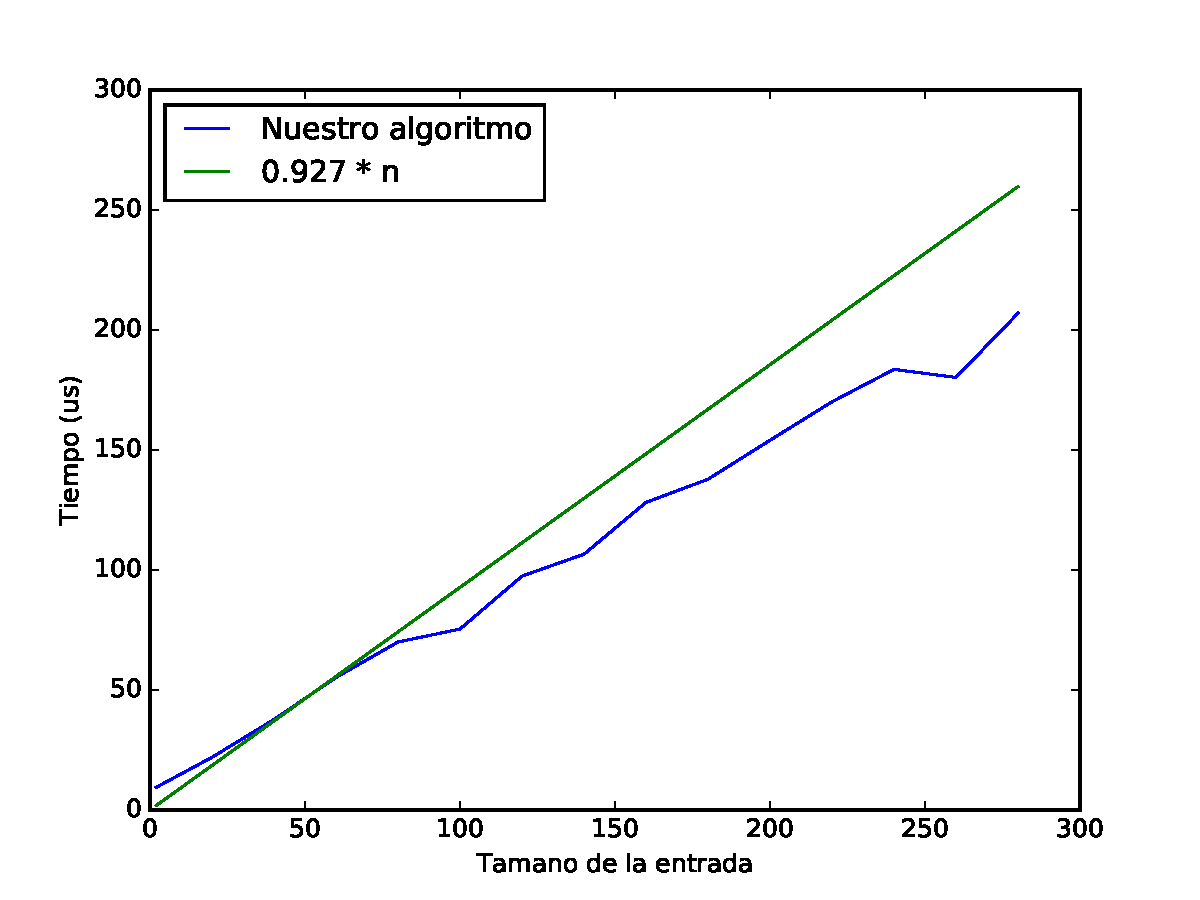
\includegraphics[width=0.9\textwidth]{img/exp/problema1-mejor.pdf}
	\caption{\footnotesize Tiempo que toma el algoritmo en $\mu$s para una entrada de tamaño $n$ ($m \in O(n))$.}
	\label{fig:problema1-mejor}
\end{figure}


Ahora veamos el caso en el que $m \in O(n^2)$. Esperaríamos que el algoritmo aquí tenga una complejidad de $O(n + m) = O(n + n^2) = O(n^2)$. Esto fue, nuevamente, confirmado experimentalmente.

\begin{figure}[H]
 \centering
	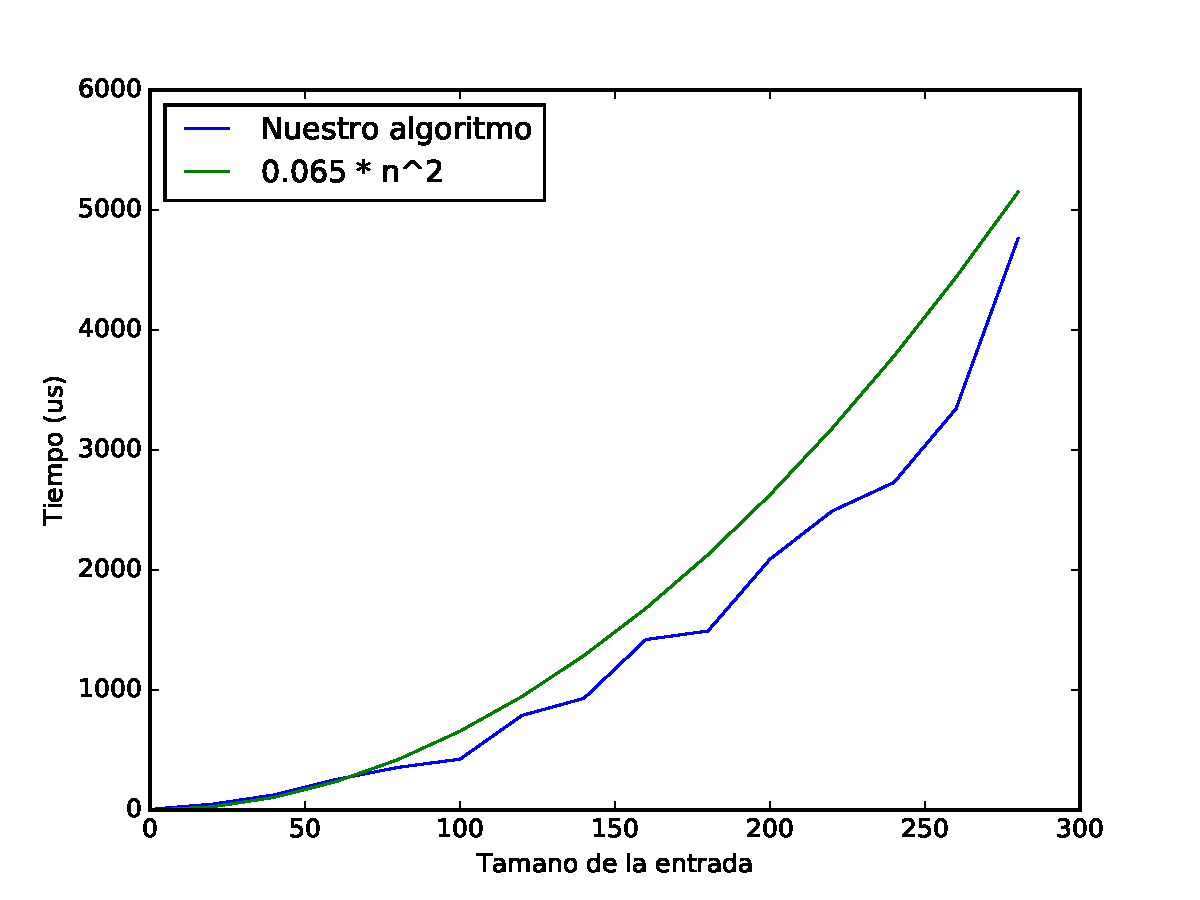
\includegraphics[width=0.9\textwidth]{img/exp/problema1-peor.pdf}
	\caption{\footnotesize Tiempo que toma el algoritmo en $\mu$s para una entrada de tamaño $n$ ($m \in O(n^2))$.}
	\label{fig:problema1-peor}
\end{figure}


Por último, como diremos en detalle en la siguiente sección, en la que explicamos la métodología de experimentación, en todos los experimentos anteriores asumimos que no importan la cantidad de caminos especiales de un grafo dado.

Esto es bastante obvio desde el punto de vista del algoritmo (pues es una consecuencia inmediata de que la complejidad esté dominada por la construcción del grafo), pero nos parece algo muy interesante verificarlo experimentalmente, dado que en este hecho se basan todos los experimentos anteriores.

Vale notar que, no obstante, sí puede haber pequeñas diferencias como consecuencia de que BFS ciertamente puede variar su performance a partir de cómo se conectan los vértices y cuántas aristas especiales hay. Pero esto afecta solo constantes, que se traducen en poco más que ruido en el gráfico.

Como puede verse en la siguiente figura, si tomamos $n$ y $m$ fijos, la cantidad de caminos especiales del grafo no afectan significativamente la performance del algoritmo.

\begin{figure}[H]
 \centering
	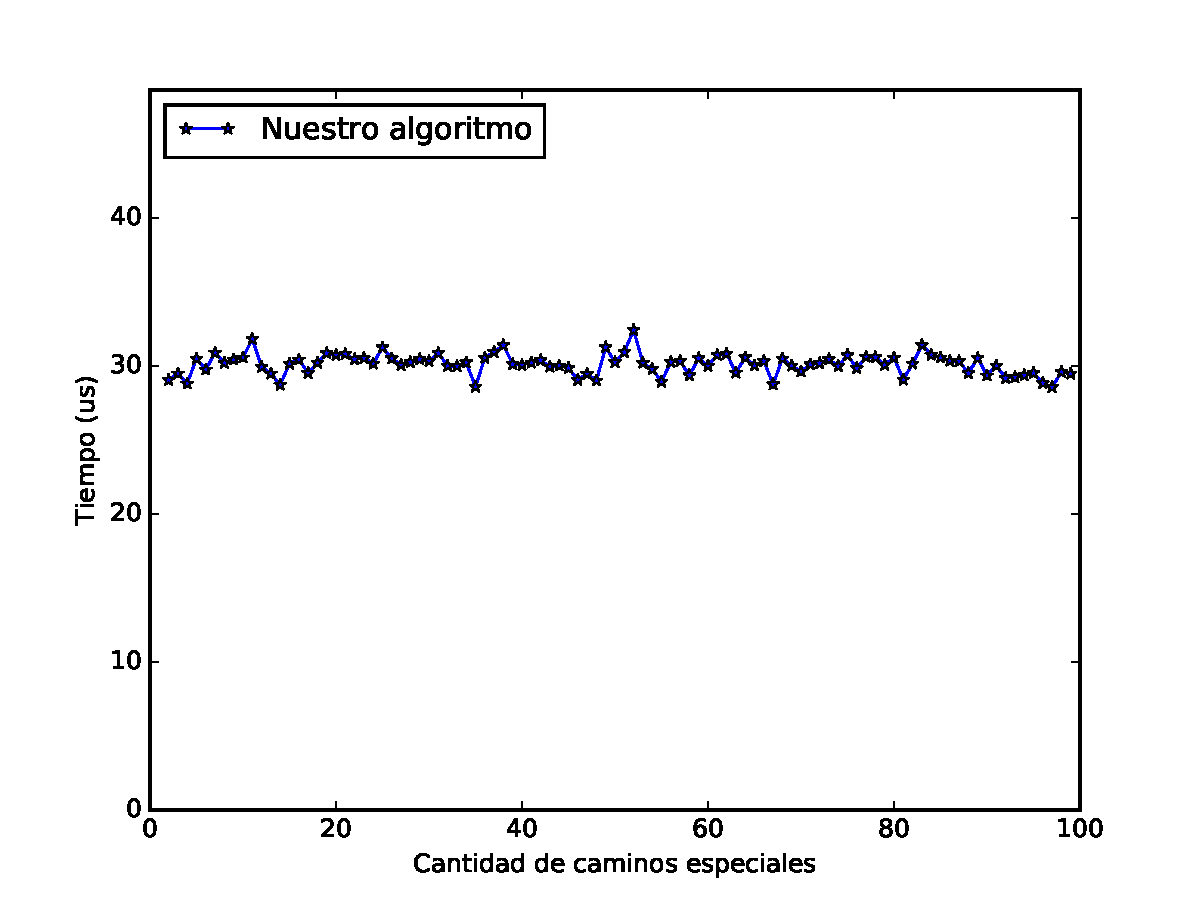
\includegraphics[width=0.9\textwidth]{img/exp/problema1-especiales.pdf}
	\caption{\footnotesize Tiempo que toma el algoritmo en $\mu$s para una entrada de tamaño $n = 15, m = 100$, variando la cantidad de caminos especiales.}
	\label{fig:problema1-especiales}
\end{figure}



\subsubsection{M\'etodo de experimentación}

Para la experimentación general del algoritmo, es decir, la verificación de que su complejidad era de $\Theta(n+m)$, generábamos distintos grafos al azar ($n$ al azar y $m$ elegido al azar tal que quede conexo).

En los casos particulares, dado $n$ fijo, tomamos $m = n - 1$ para el primer experimento y $m = \frac{n (n - 1)}{2}$ en el segundo.

Para la generación al azar de grafos utilizamos el algoritmo descripto en la sección \ref{subsec:grafos-aleatorios} del apéndice. Vale la pena aclarar cómo hicimos para decidir cuántas aristas especiales tendría el grafo. Primero, lo que hicimos fue notar experimentalmente que, con $n$ y $m$ fijos, si tomábamos distinta cantidad de caminos especiales (de 2 a $m$), la varianza de las mediciones era muy baja, es decir, la cantidad de caminos especiales de un grafo no afecta a la performance. 

Esto fue observado y comprobado experimentalmente. En consecuencia, para cada $n$ y $m$ fijo, tomamos grafos totalmente al azar, con cantidad de caminos especiales también al azar, y calculamos la mediana de todos los tiempos para determinar el tiempo total.

